\documentclass[12pt,a4paper,twoside]{article}

\usepackage[a4paper,left=2.2cm,right=2.2cm,bottom=2.5cm,top=2.5cm,footskip=32pt]{geometry}
\usepackage{setspace}
\usepackage{time}
\usepackage[sort]{natbib}
\usepackage{graphicx}
\usepackage{amsmath,amssymb,bm}
% \usepackage[dvipsnames]{xcolor}
\usepackage[table,xcdraw,dvipsnames]{xcolor}
\usepackage{hyperref}
\usepackage{multirow}
\usepackage{cleveref}

\usepackage{epigraph}
\setlength{\epigraphwidth}{2.9in}
\usepackage{authblk}
\newsavebox\CBox
\def\textBF#1{\sbox\CBox{#1}\resizebox{\wd\CBox}{\ht\CBox}{\textbf{#1}}}

\newcommand\myshade{85}
\colorlet{mylinkcolor}{violet}
\colorlet{mycitecolor}{YellowOrange}
\colorlet{myurlcolor}{Aquamarine}

\hypersetup{
	linkcolor  = mylinkcolor!\myshade!black,
	citecolor  = mycitecolor!\myshade!black,
	urlcolor   = myurlcolor!\myshade!black,
	colorlinks = true,
}

\usepackage{fancyhdr}
\usepackage[printwatermark]{xwatermark}
%\newwatermark[allpages,color=gray!50,angle=45,scale=1.5,xpos=0,ypos=0]{Draft. Do not circulate or cite}

\begin{document}%Data and Methods
	
\title{\normalsize{Main draft}\\
	$\,$\\	$\,$\\
	\begin{Huge}
		Option 1: Forecasting vital rates from demographic summary measures \linebreak
		
		Option 2: Demographic forecasting from summary measures 
	\end{Huge}}


	\author[1]{Carlo G.~Camarda\thanks{Corresponding author: \url{carlo-giovanni.camarda@ined.fr}\\
		\hspace*{1.8em}Address: 9 cours des Humanités, 93322 Aubervilliers - France}}
\author[2]{Jos\'e Manuel Aburto}
\affil[1]{\small \textit{Institut national d'\'{e}tudes d\'emographiques (INED)}}
\affil[2]{\small \textit{Leverhulme Centre for Demographic Science, Department of Sociology and Nuffield College at  \authorcr \textit{ University of Oxford; CPop at University of Southern Denmark}}}


\date{}
\maketitle
\thispagestyle{empty}

\pagestyle{fancy}
\fancyhead[RO,LE]{\small}
\fancyhead[LO]{\small Camarda \& Aburto: Forecasting vital rates from summary measures}% odd page header and number to right top
\fancyhead[RE]{\small Submitted to the IPC 2021}%Even page header and number at left top
\fancyfoot[L,R,C]{}
\rfoot{\thepage}

	
	
	\begin{abstract}
In population and actuarial sciences, time-trends of summary measures (such as life expectancy or the average number of children per woman) are easy to interpret and predict. Most summary measures are nonlinear functions of the vital rates, the key variable we usually want to estimate and forecast. Furthermore smooth outcomes of future age-specific vital rates are desirable. Therefore, optimization with nonlinear constraints in a smoothing setting is necessary. We propose a methodology that combines Sequential Quadratic Programming and a $P$-spline approach, allowing to forecast age-specific vital rates when future values of demographic summary measures are provided. We provide an application of the model on Italian mortality and Spanish fertility data.
\\
\\$\,$\\
{\bf Keywords:} Vital rates forecast; Smoothing; Constrained nonlinear optimization; Summary measures.
	\end{abstract}
	
%	\keywords{} 
	
	
	
	%%%%%--------------------------------------%%%%%%%%%%%%%%%%%%%
	%%%%%--------------------------------------%%%%%%%%%%%%%%%%%%%

	\newpage
	\pagenumbering{arabic} 
\setcounter{page}{1}	

\section{Introduction}\label{sec:Intro}

Demographic forecasting is a key research element in population dynamics and in demography. Reliable estimates of future vital rates are important because they are essential for social and economic planning. Mortality and fertility are often predicted by modelling and extrapolating rates over age and time \citep{Booth2006,bohk2018forecast}. However, the high dimensionality, especially when using single years of age, is a major challenge for age-specific forecasting. Forecasting summary measures such as life expectancy at birth (e.g. \citet{pascariu2018double}) or the average number of children that a group of women will have over their reproductive lifespans (e.g. \citet{alkema2011probabilistic}) has the advantage of dealing with a single (or few) time series, but then the challenge is to derive reliable age-specific estimates from these forecasts. 

In the past, a target summary measure (e.g. life expectancy at birth) was set and model life or fertility tables would provide the target age-specific vital rates \citep{Booth2006}. More recently, \citet{vsevvcikova2016age} derived full age specific vital rates consistent with the United Nations probabilistically projected values of life expectancy at birth and period total fertility rate (TFR) \citep{gerland2014WorldPopulationStabilization}. To estimate age-specific death rates, they developed a methodology based on back engineering the Lee-Carter forecasting model \citep{lee1992modeling}. Subsequently, future age patterns of fertility, consistent with the projected TFR, were derived interpolating between a starting age pattern of fertility and a target model pattern. In more recent work, \citet{pascariu2020linear} leveraged the high correlation between life expectancy and death rates across ages to estimate a full mortality profile from values of life expectancy at birth. These methodologies aim at deriving age-specific vital rates from one summary indicator. A key question is whether results from these models provide reliable estimates that are consistent with complementary indicators such as lifespan inequality or the variation in age-specific fertility rates. 

Previous evidence in mortality research suggests that standard methodologies based on forecasting age-specific death rates and rates of mortality improvements provide accurate values for life expectancy but not necessarily for measures of dispersion in ages at death \citep{bohk2017lifespan}. In fertility, information about other summary measures besides TFR such as the variance of reproductive outcomes is often neglected \citep{hruschka2016does}. A notable exception in fertility research was made by \citet{thompson1989multivariate}, who forecast the total fertility rate, the mean age at childbearing, and the standard deviation of the age at childbearing and retrieved age-specific fertility rates relying on the gamma distribution. Aiming at filling this gap in development of forecasting methodologies, we propose a model to derive future mortality and fertility age-patterns complying with projected summary measures of central tendency (e.g. life expectancy and TFR) and dispersion (e.g. lifespan inequality and variance in age at childbearing). 

Unlike comparable approaches, we assume only smoothness of future vital rates, which is achieved by a two-dimensional $P$-spline approach as in \citet{currie2004smoothing}, and we allow constraints to multiple series of summary measures. Since these measures are commonly nonlinear functions of the estimated penalized coefficients, Lagrangian multipliers cannot be directly implemented. We hence opted for a Sequential Quadratic Programming (SQP) procedure \citep{nocedal2006sequential} to perform the associated constrained nonlinear optimization.
We illustrate our approach with two data sets. We forecast mortality of Italian females, based on future life expectancy predicted by \citet{UN2019} and a future trend of a lifespan disparity measure obtained by time-series analysis. We also forecast Spanish fertility constrained to future values of total fertility rates, mean and variance of age at childbearing, derived by time-series analysis.

\section{Methodology}

\subsection{Data}
We use data on deaths and population counts from the World Population Prospects for Italian females from 1960-1965 to the latest period 2010-2015 available. To test our model we use the projected life expectancy to 2050 and estimated future values for lifespan disparity using standard time series techniques with the projected death and population counts \citep{UN2017}. We also apply our model to fertility. For this we use data from the World Population Prospects for the total fertility rate (TFR) \citep{UN2017}, and age-specific births and population from the Human Fertility Database for Spanish females \cite{HFD}.


\section{Model on Italian mortality data}

For ease of presentation, we formulate the model on mortality data. We suppose that we have deaths, and exposures to risk, arranged in two matrices, 
$\bm{Y} = (y_{ij})$ and $\bm{E} = (e_{ij})$, each $m \times n_{1}$, whose rows and columns are classified by age at death, $\bm{a}, \,m \times 1$, and year of death, $\bm{t}_{1}, \,n_{1} \times 1$, respectively.  
We assume that the number of deaths $y_{ij}$ at age $i$ in year $j$ is Poisson distributed with mean $\mu_{ij} \,e_{ij}$. %The value of $\mu_{ij}$ is commonly named force of mortality. 
Forecasting aims to reconstruct trends in $\mu_{ij}$ for $n_{2}$ future years, $\bm{y}_{2}, n_{2} \times 1$.

It is common practice to summarize mortality age-patterns by computing measures such as life expectancy at birth ($e_{0}$) and lifespan disparity measures. Time-trends of these summary measures are often regular and well-understood. Forecasting these time-series is therefore an easier task. Figure~\ref{fig:CamardaMort} (top-left panel) presents observed $e_{0}$ for Italian females from 1960 to 2016 along with the medium variant up to 2050 as computed by the UN. A second constraint is given by future values of $e^{\dagger}$, a lifespan disparity measure defined as the average years of life lost in a population attributable to death \citep{VaupelCRdemo2003}. Future values of this measure are obtained by conventional time-series models and portrayed in the top-right panel of Figure~\ref{fig:CamardaMort}. Future mortality patterns, both by age and over time, must adhere to these predicted trends.

\begin{figure}[!ht]\centering
	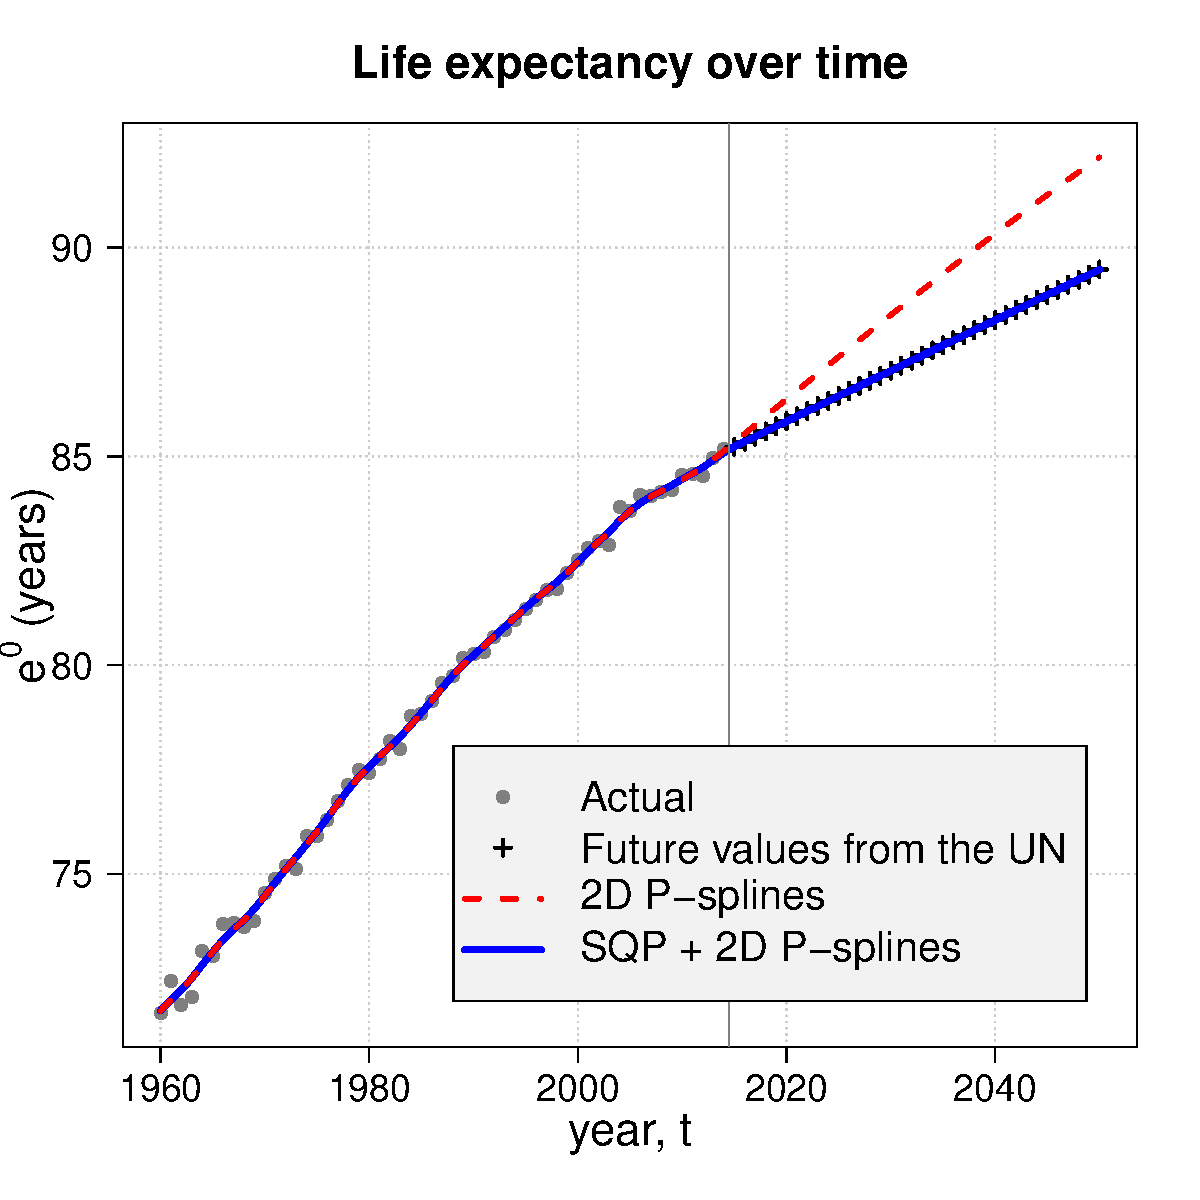
\includegraphics[scale=0.35]{./Figures/Camardafig1a.pdf}
	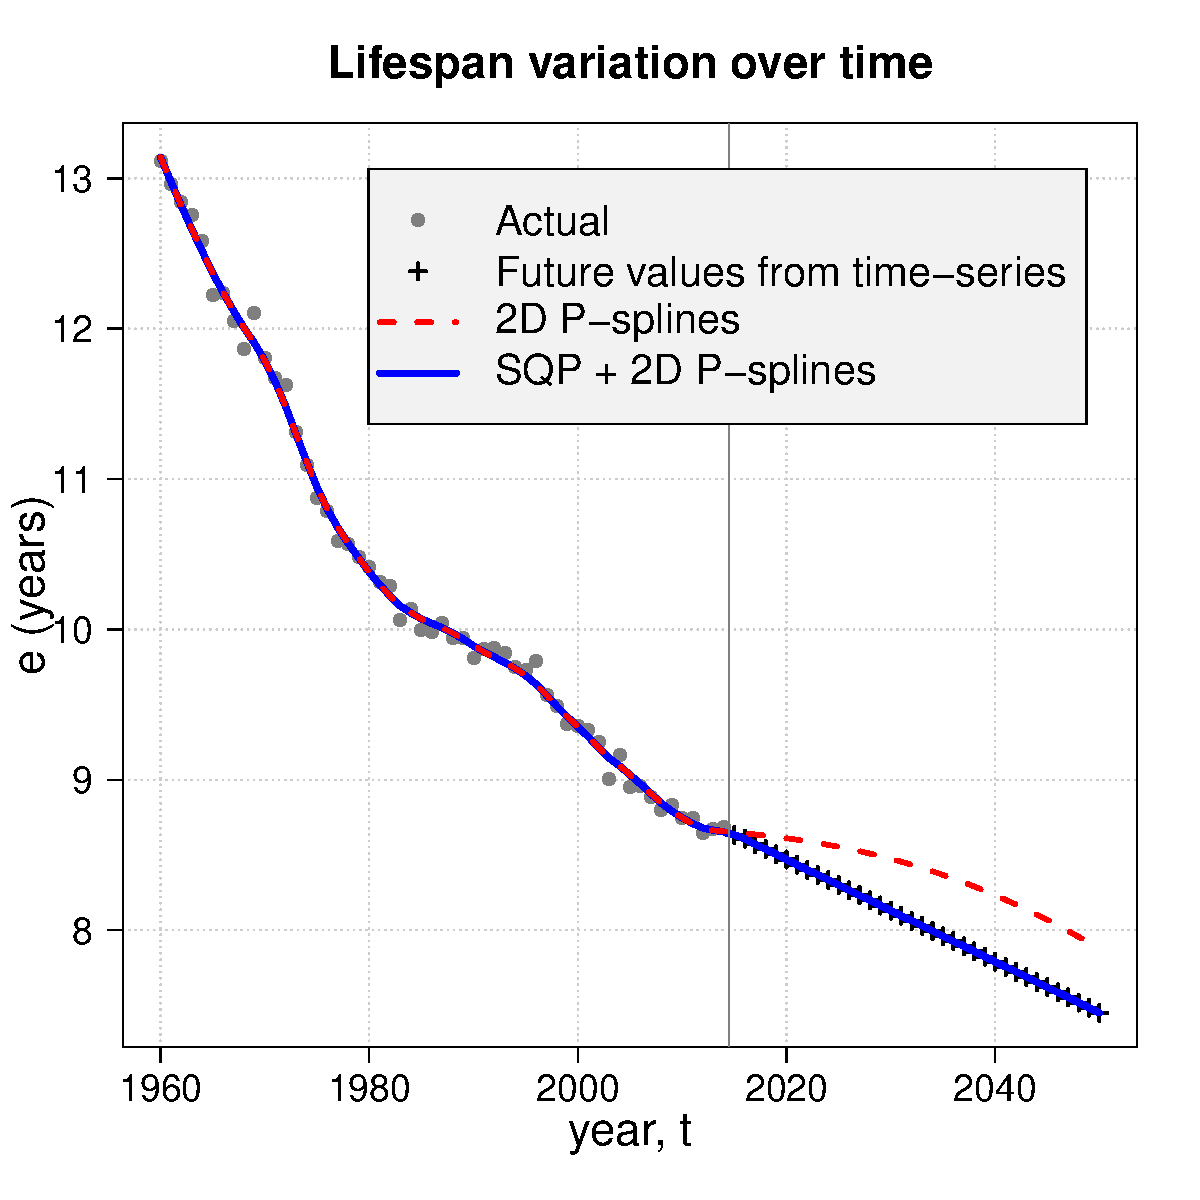
\includegraphics[scale=0.35]{./Figures/Camardafig1b.pdf}
	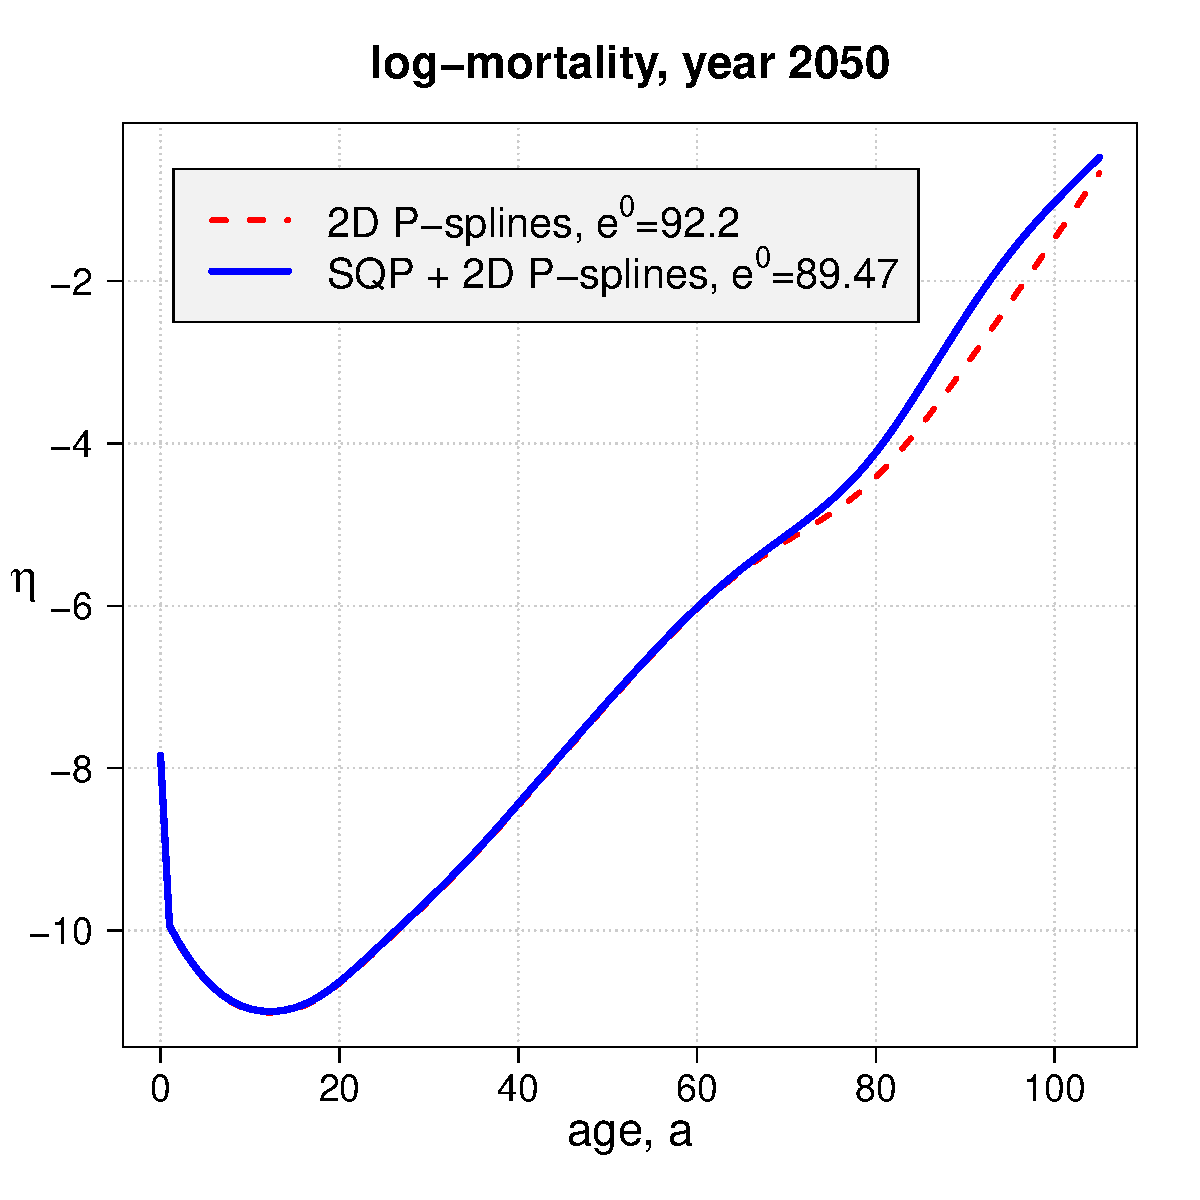
\includegraphics[scale=0.35]{./Figures/Camardafig1c.pdf}
	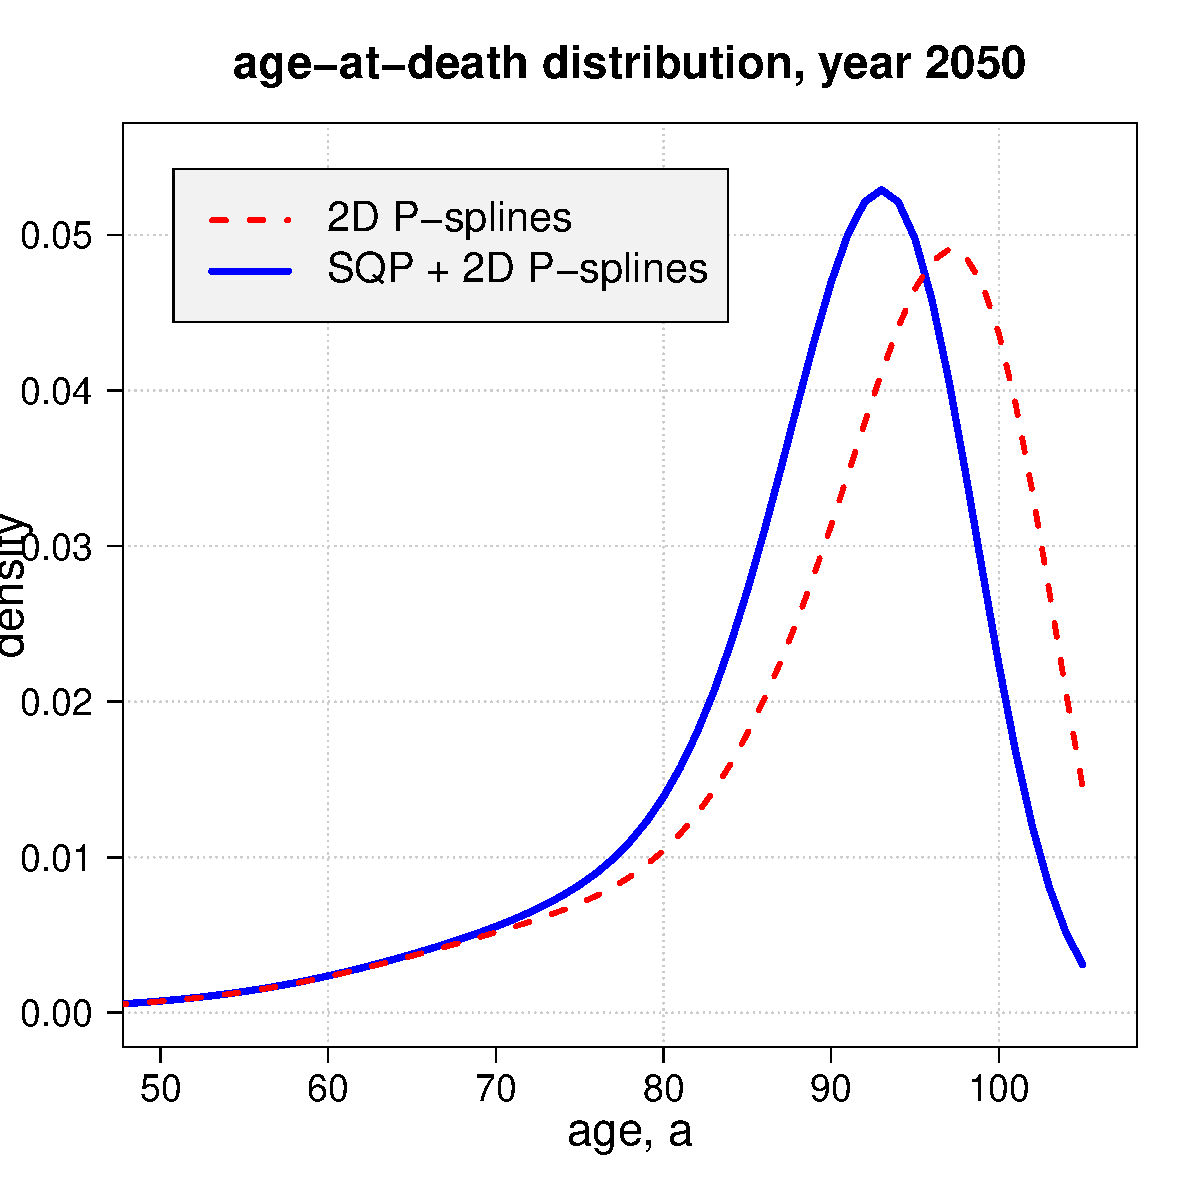
\includegraphics[scale=0.35]{./Figures/Camardafig1d.pdf}
	\caption{\label{fig:CamardaMort} Top panels: Actual, estimated and forecast life expectancy at birth and lifespan disparity measure by United Nations and time-series, 2D $P$-splines and the SQP+2D $P$-splines. Bottom panels: Mortality in 2050 described by log-hazards and associated densities (ages 50+) by 2D $P$-splines and the SQP+2D $P$-splines. Italian females, ages 0-105, years 1960-2014, forecast up to 2050.}
\end{figure}

We arrange data as a column vector, that is, $\bm{y} = \verb"vec"(\bm{Y})$ and $\bm{e} = \verb"vec"(\bm{E})$ and we model our Poisson death counts as follows: $\ln(E(\bm{y})) = \ln(\bm{e})+ \bm{\eta} = \ln(\bm{e})+ \bm{B}\,\bm{\alpha}\, , $ where $\bm{B}$ is the regression matrix over the two dimensions: $\bm{B} = \bm{I}_{n_{1}} \otimes \bm{B}_{a}$, with $\bm{B}_{a} \in \mathbb{R}^{m \times k_{a}}$. Over time, we employ an identity matrix of dimension $n_{1}$ because we will incorporate a constraint for each year. Over age, $\bm{B}_{a}$ includes a specialized coefficient for dealing with mortality at age 0. In order to forecast, data and bases are augmented as follows:
\begin{equation}\label{eq:AugData}
\breve{\bm{E}} = [\bm{E} : \bm{E}_{2}]\, , \qquad 
\breve{\bm{Y}} = [\bm{Y} : \bm{Y}_{2}]\, , \qquad
\breve{\bm{B}} = \bm{I}_{n_{1}+n_{2}} \otimes \bm{B}_{a}
\, ,
\end{equation}
where $\bm{E}_{2}$ and $\bm{Y}_{2}$ are filled with arbitrary future values. If we define a weight matrix $\bm{V} = \mathrm{diag}(\verb"vec"(\bm{1}_{m\times n_{1}}:\bm{0}_{m\times n_{2}}))\,$, the coefficients vector $\bm{\alpha}$
can be estimated by a penalised version of the iteratively reweighted least squares algorithm: 
\begin{equation}\label{eq:penIRWLSfor}
(\breve{\bm{B}}' \bm{V} \tilde{\bm{W}} \breve{\bm{B}} + \bm{P}) \tilde{\bm{\alpha}} =
\breve{\bm{B}}'\bm{V} \tilde{\bm{W}}\tilde{\bm{z}} \, ,
\end{equation} 	
where a difference penalty $\bm{P}$ enforces smoothness behaviour of mortality both over age and time. Outcomes from this approach in terms of life expectancy and $e^{\dagger}$ are depicted with a dashed line in Figure~\ref{fig:CamardaMort} (top panels), and departures from the UN and time-series projected values are evident. 

Both life expectancy and average years of life lost are nonlinear function of the coefficients vector $\bm{\alpha}$. For a year $j$ and associated $k_{a}$ coefficients $\bm{\alpha}_{j}$, we denote mortality by $\bm{\mu}_{j} = \exp(\bm{B}_{a}\bm{\alpha}_{j})$. We can write our summary measures as follows
\begin{eqnarray}\label{eq:e0ed}
e^{0} (\bm{\alpha}_{j}) &=& \;\;\,\,\bm{1}_{m}' \, \exp[ \bm{C} \, \bm{\mu}_{j}]  + 0.5 \\
e^{\dagger} (\bm{\alpha}_{j}) &=&  - \exp[ \bm{C} \, \bm{\mu}_{j}]' \, \bm{C} \bm{\mu}_{j} \nonumber
\end{eqnarray} 
where $\bm{C}$ is a $(m \times m)$ lower triangular matrix filled only with -1. 

%\begin{equation}\label{eq:Cmat}
%\bm{C} = \left[\begin{array}{rrrr}
%-1 & 0 & \cdots & 0 \\
%-1 & -1& \cdots & 0 \\
%\vdots & \vdots & \ddots & \vdots \\
%-1 & -1 & \cdots & -1
%\end{array}\right] \, .
%\end{equation}

Constrained nonlinear optimization is therefore	necessary and a SQP approach is implemented. Let denote with $\bm{N}^{0}$ and $\bm{N}^{\dagger}$ the $(k_{a}n_{2} \times n_{2})$ matrices with block-diagonal structures containing derivatives of~\eqref{eq:e0ed} with respect to $\bm{\alpha}_{j}$ for $j=n_{1}+1, \ldots n_{1}+n_{2}$:
\begin{eqnarray}\label{eq:Der}
\frac{\partial e^{0} (\bm{\alpha}_{j})}{\partial \bm{\alpha}_{j}} &=& \bm{1}_{m}' \verb"diag"[\exp(\bm{C}\bm{\mu}_{j})] \,	\bm{C} \,\verb"diag"(\bm{\mu}_{j}) \bm{B}_{a}\\
\frac{\partial e^{\dagger} (\bm{\alpha}_{j})}{\partial \bm{\alpha}_{j}} &=& - \bm{B}_{a}' \left\{ \bm{C}'[\bm{C}\bm{\mu}_{j} \circ \exp(\bm{C}\bm{\mu}_{j})] \circ \bm{\mu}_{j} \right\} + \nonumber\\
&& - \bm{B}_{a}' \left\{ [\bm{C}' \exp(\bm{C}\bm{\mu}_{j})] \circ \bm{\mu}_{j} \right\} \nonumber\, ,
\end{eqnarray}
where $\circ$ represents element-wise multiplication. Target life expectancy and lifespan disparity for future years are given by $n_{2}$-vectors $\bm{e}^{0}_{\mathrm{T}}$ and $\bm{e}^{\dagger}_{\mathrm{T}}$.

Solution of the associated system of equations at the step $\nu + 1$ is given by
\begin{equation}\label{eq:SQLalg}
\left[ \begin{array}{l}
\bm{\alpha}_{\nu+1}\\
\bm{\omega}_{\nu+1}
\end{array}\right] = 
\left[ \begin{array}{lllll}
\bm{L}_{\nu}  &:& \bm{H}^{0}_{\nu} &:& \bm{H}^{\dagger}_{\nu}\\
\bm{H}_{\nu}^{0 T}  &:& \bm{0}_{n_{2} \times n_{2}}&:&\bm{0}_{n_{2} \times n_{2}}\\
\bm{H}_{\nu}^{\dagger T} &:& \bm{0}_{n_{2} \times n_{2}} &:& \bm{0}_{n_{2} \times n_{2}}
\end{array}\right]^{-1}
\left[ \begin{array}{c}
\bm{r}_{\nu} - \bm{L}_{\nu}\bm{\alpha}_{\nu}\\
\bm{e}^{0}_{\mathrm{T}} - \bm{e}^{0} (\bm{\alpha}_{\nu})\\
\bm{e}^{\dagger}_{\mathrm{T}} - \bm{e}^{\dagger} (\bm{\alpha}_{\nu})\\
\end{array}\right] \, ,
\end{equation}
where $\bm{L}$ and $\bm{r}$ are left- and right-hand-side of the system in~\eqref{eq:penIRWLSfor}, and matrices $\bm{H}^{0} = \left[\bm{0}_{k_{a}n_{1}\times n_{2}}:\bm{N}^{0} \right]'$ and $\bm{H}^{\dagger} = \left[\bm{0}_{k_{a}n_{1}\times n_{2}}:\bm{N}^{\dagger} \right]'$. Vector of $\bm{\omega}$ denotes the current solution of the associated Lagrangian multipliers for both set of constraints.

Future values for $e^{0}$ and $e^{\dagger}$ forecast by the proposed method are exactly equal to the UN and time-series values (Figure~\ref{fig:CamardaMort}, top panels). The bottom panels show the forecast mortality age-pattern in 2050: the shape obtained by the suggested approach is not a simple linear function of the plain $P$-splines outcome, and differences are evident by looking at the associated age-at-death distributions. 

\section{Spanish Fertility Data}

We forecast Spanish fertility using three commonly-used summary measures: Total Fertility Rate describing average number of children per women in a given year, and mean and variance of childbearing age which measure fertility shape over age. In formulas:
\begin{eqnarray}\label{eq:FertMea}
TFR(\bm{\alpha}_{j}) &=& \bm{1}_{m}' \, \bm{\mu}_{j}\\
MAB(\bm{\alpha}_{j}) &=& \bm{\mu}_{j}' \, (\bm{a}+0.5) \; / \; TFR(\bm{\alpha}_{j})\nonumber\\
VAB(\bm{\alpha}_{j}) &=& \bm{\mu}_{j}' \, (\bm{a}+0.5)^2 \; / \; TFR(\bm{\alpha}_{j}) - MAB(\bm{\alpha}_{j})^2\nonumber \, .
\end{eqnarray} 

We forecast trends of these measures by time-series analysis. We then smooth and constrain future fertility age-patterns to comply forecast values of \eqref{eq:FertMea} as in \eqref{eq:SQLalg}. Summary measures as well as fertility rates in 2050 are presented in Figure~\ref{fig:CamardaFert}. Differences between proposed approach and plain 2D $P$-splines are clear. Whereas $P$-splines blindly extrapolate previous trends mainly accounting for the last observed years, the proposed approach enforces future age-patterns to adhere combinations of summary measures, guiding future fertility toward demographic meaningful trends. 

\begin{figure}[!ht]\centering
	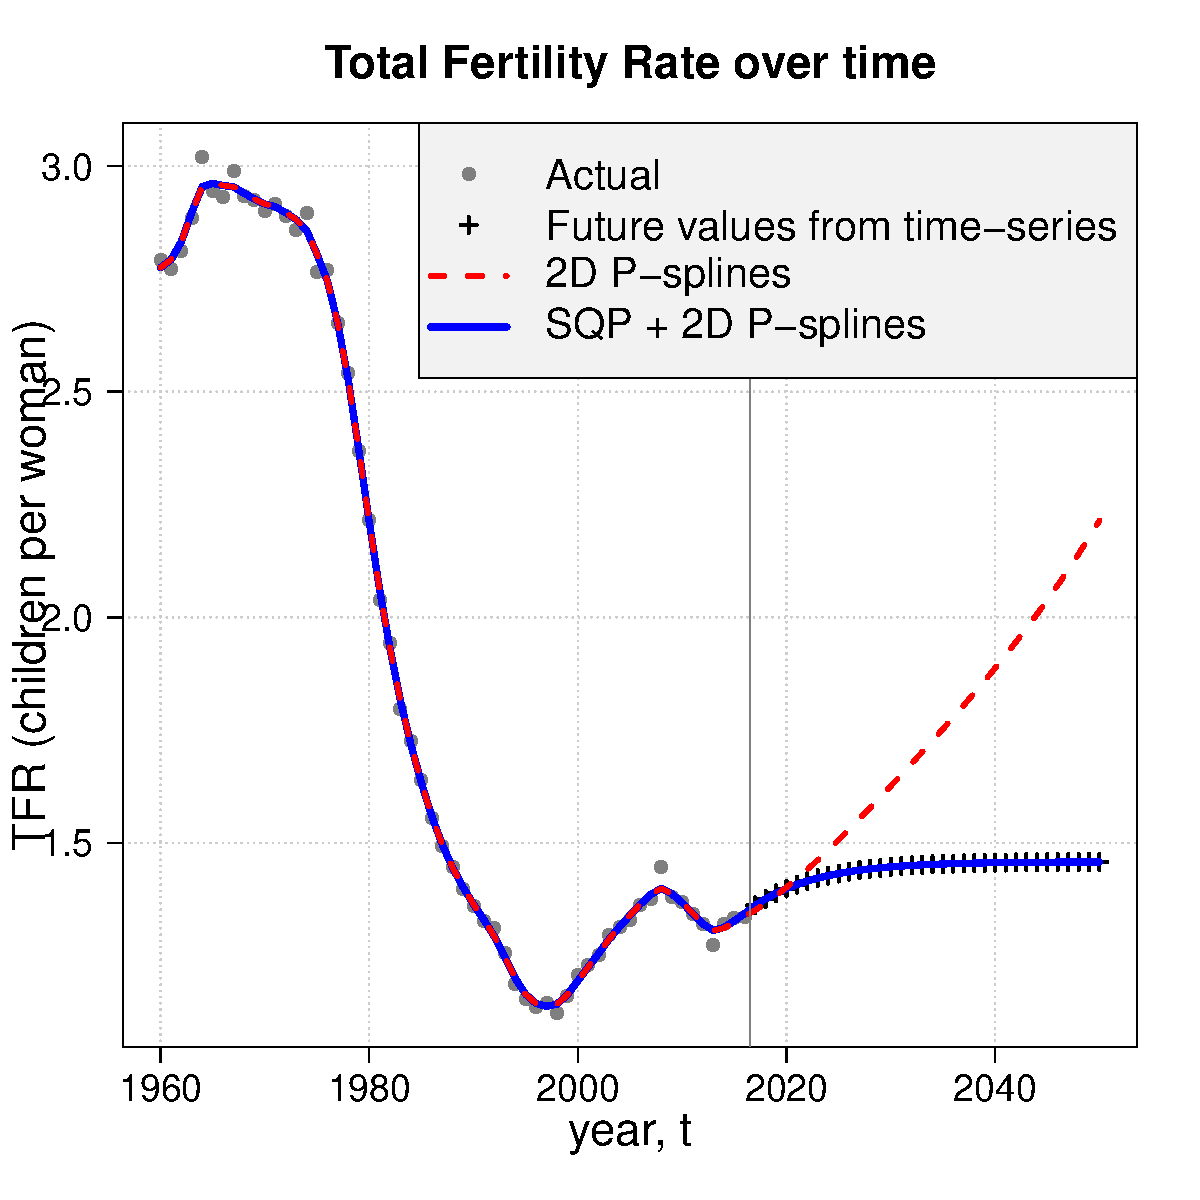
\includegraphics[scale=0.35]{./Figures/Camardafig2a.pdf}
	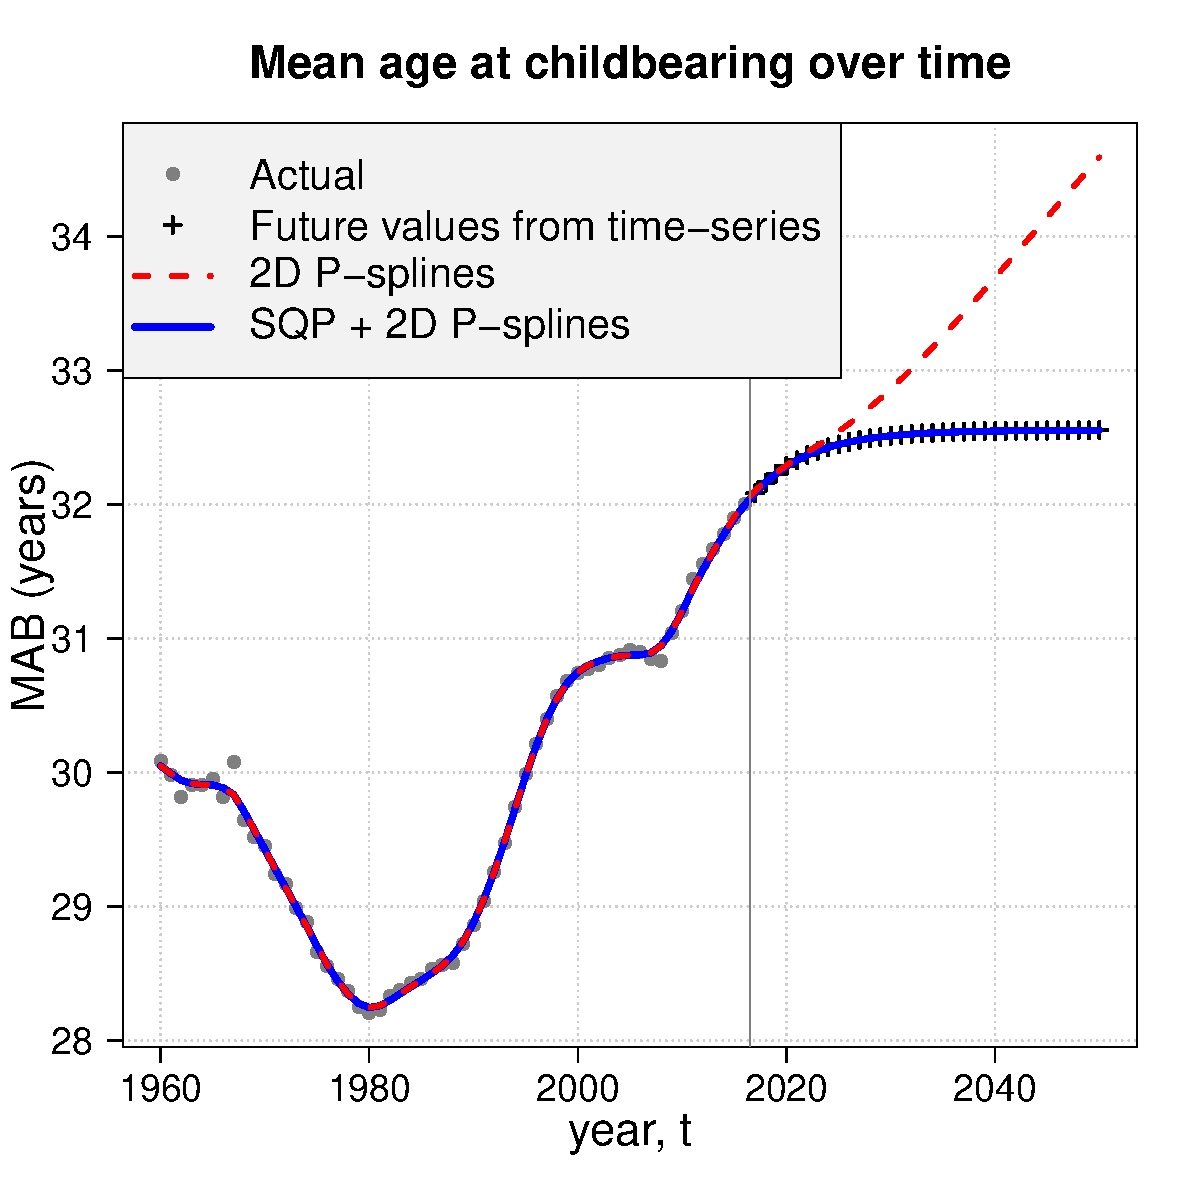
\includegraphics[scale=0.35]{./Figures/Camardafig2b.pdf}
	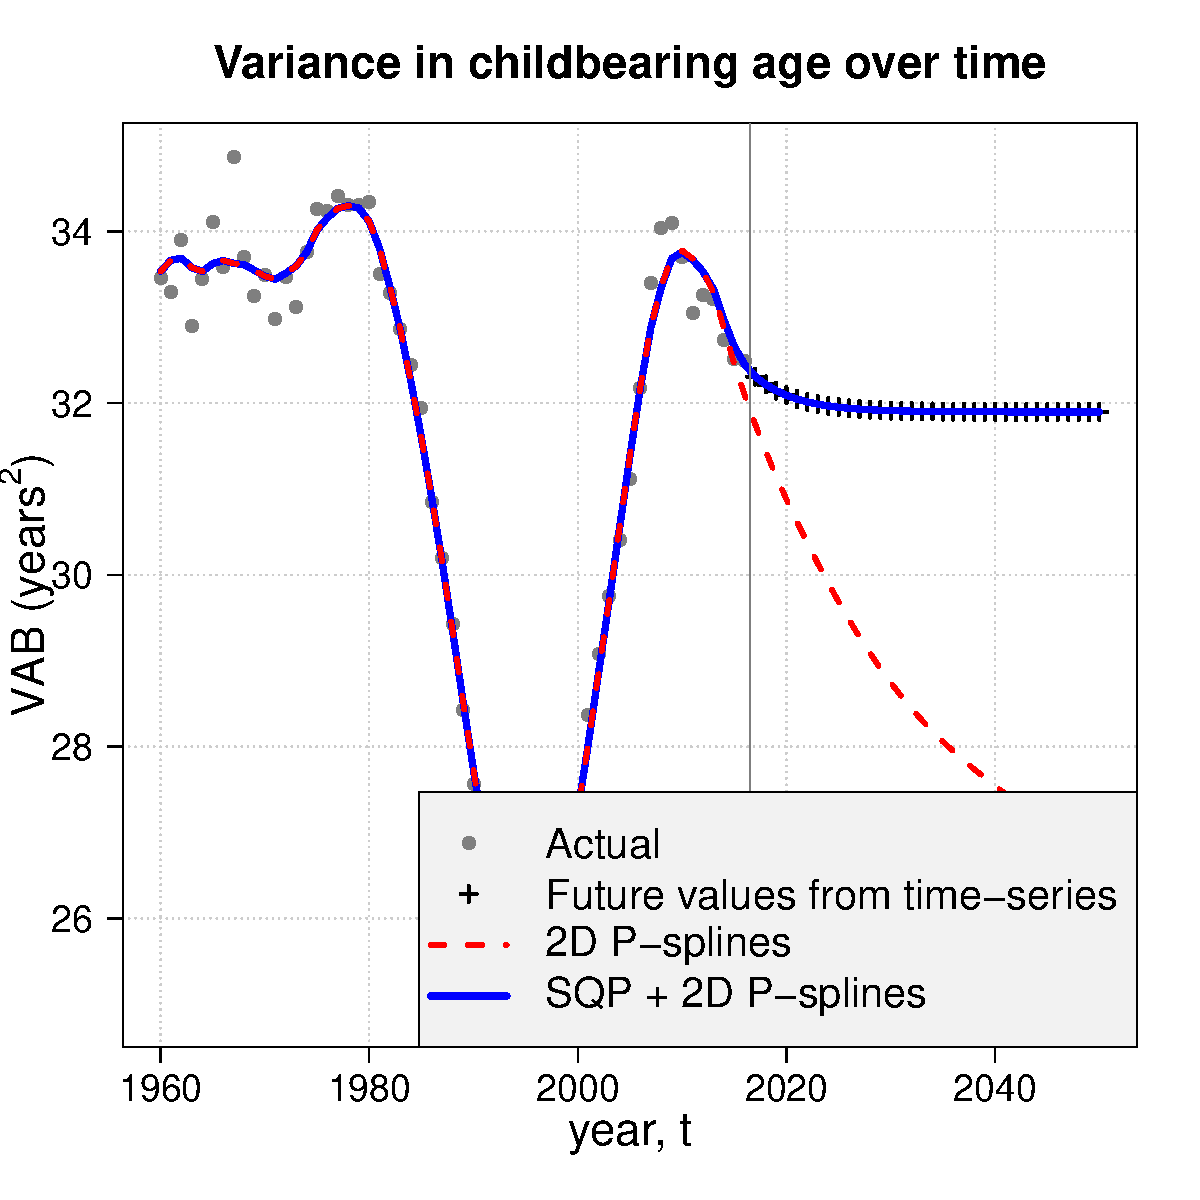
\includegraphics[scale=0.35]{./Figures/Camardafig2c.pdf}
	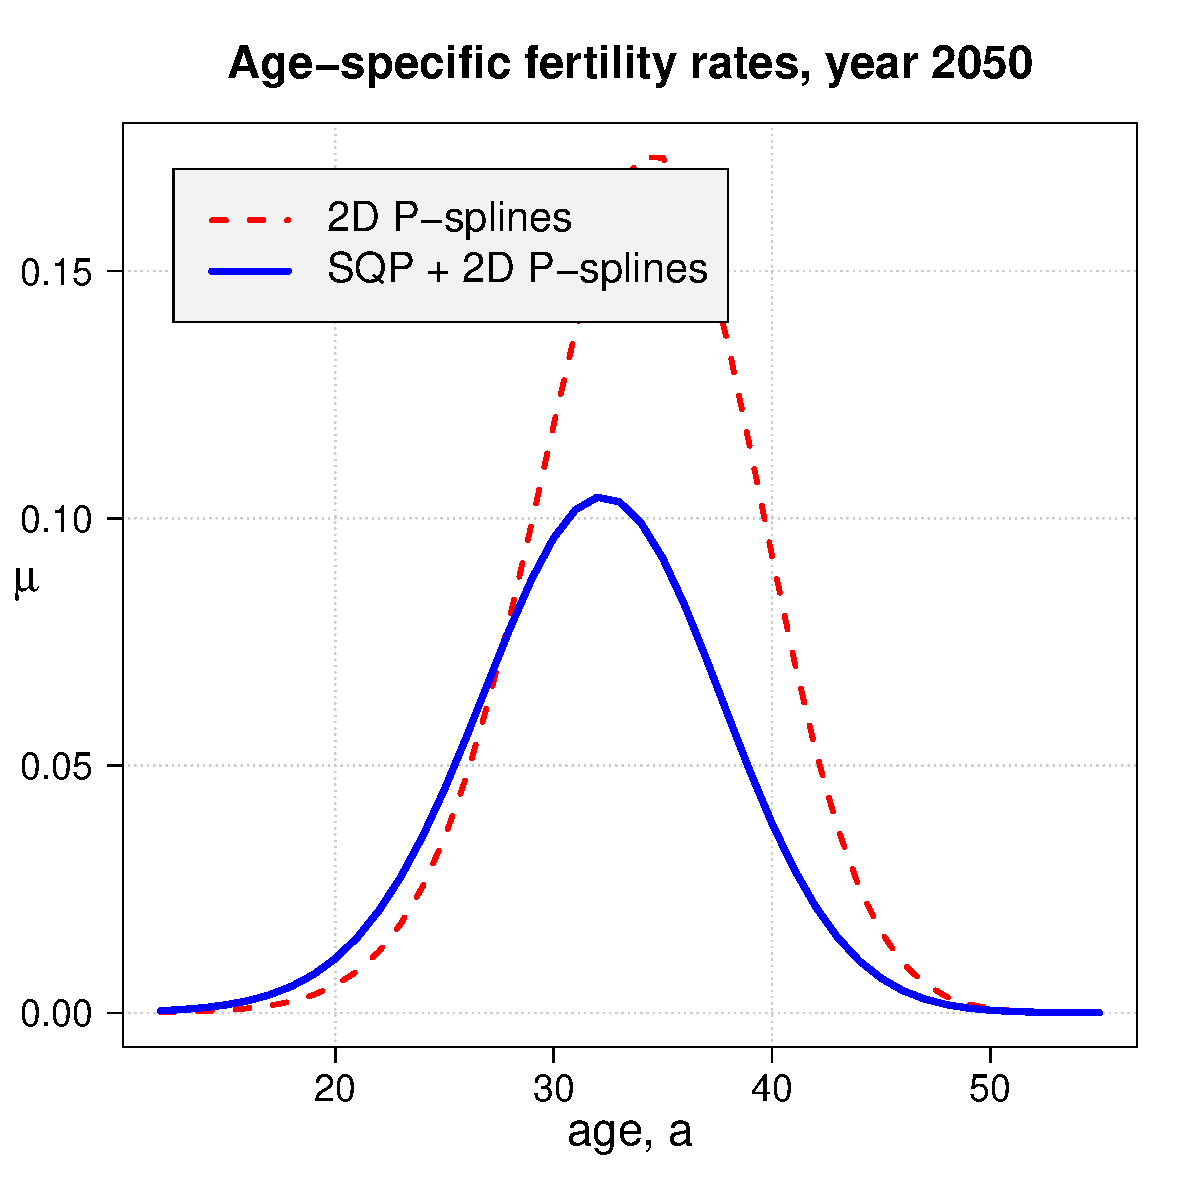
\includegraphics[scale=0.35]{./Figures/Camardafig2d.pdf}
	\caption{\label{fig:CamardaFert} Top and left-bottom panels: Actual, estimated and forecast Total Fertility Rate, Mean and Variance in childbearing age by time-series analysis, 2D $P$-splines and the SQP+2D $P$-splines. Right-bottom panel: Age-specific fertility rate in 2050 by 2D $P$-splines and the SQP+2D $P$-splines. Spain, ages 12-55, years 1960-2016, forecast up to 2050.}
\end{figure}


\section{Discussion}



\section*{Appendix A}

The Gini coefficient is an indicator of relative variation. It was originally proposed in Economics to measure income or wealth inequality and  has been adopted in demography and survival analysis to measure lifespan variation \citep{Hanada1983,Shkolnikov2003,bonetti2009gini,gigliarano2017longevity} There exist several alternative and equivalent ways to define the Gini coefficient \citep{yitzhaki2013gini}. For our purposes and the remainder of this article, we will use the following formulation: 
%
\begin{equation}\label{eq:G}
G(\bm{\alpha}_{j}) = \bm{1}_{m}^{T} - \frac{ \bm{1}_{m}^{T} \, \exp[ 2\, \bm{C} \, \bm{\mu}_{j}] }{e^{0} (\bm{\alpha}_{j})}, 
\end{equation}
%
which is equivalent to $G = 1-\frac{\int_0^\infty\ell(x)^2\,dx}{\int_0^\infty\ell(x)\,dx}$ \citep{michettid1957,Hanada1983}.
Where $\int_0^\infty \ell(x)^2\,dx$ is the resulting life expectancy at birth of doubling the hazard at all ages. The Gini coefficient takes values between 0 and 1. A coefficient equal to 0 corresponds to the case of perfect equality in ages at death. The Gini index increases as lifespans become more spread and unequal in the population, reaching a value of 1 in the case of perfect inequality.



% Line interpsace
\linespread{1}\normalsize

% Font size
\small

% References
\bibliographystyle{apa}
\bibliography{Bib_FertMort}

\end{document} 

%For example, in developed countries, the linear increase in life expectancy over some periods has made it easier to fit trends over time of this summary indicator than fitting more complex models based on age-specific dynamics of mortality \citep{White200259}. Therefore, several methods have been proposed to forecast life expectancy. For instance, \citet{torri2012forecasting} forecast life expectancy for a given country assuming a tendency towards a predicted best practice life expectancy. \citet{pascariu2018double} proposed incorporating the analysis of the gap between female and male life expectancy to more accurately predict the overall level of mortality in a country. Similarly, \citet{Raftery2013} forecast life expectancy for several countries using a Bayesian hierarchical model for females, and then model the sex gap to estimate male life expectancy \citep{raftery2014joint}. Subsequently, the overall level of mortality given by life expectancy is converted to a age-specific profile \citep{vsevvcikova2016age}. This latter method has been adopted by the United Nations. However, life expectancy, as an average, conceals the variation in the age-at-death distribution \citep{van2018case}. While the sources of variance in lifespans, or the health inequalities it reflects, are not fully understood, they however are a key problem for policy as well for modelling and forecasting mortality \citep{tuljapurkar2011variance}.

% Recently, \citet{bohk2017lifespan} proposed to incorporate the variation in ages at death as an additional indicator to evaluate mortality forecast. This variation is often called lifespan variation or lifespan inequality and refers to how similar ages at death are in a population. They found that some methods struggle to account for trends in lifespan variation, which results in a mismatch between life expectancy and lifespan variation. In most countries, life expectancy and lifespan variation are often negatively correlated \citep{Smits2009,Vaupel2011,colchero2016emergence, alvarez2019latin, gonzaga2018compression}, however in some countries this association is less strong when looking at first differences over time. For example, in Central and Eastern European countries and in some Latin American countries life expectancy and lifespan variation moved independently from each other in periods when life expectancy improvements slowed-down \citep{Aburto2018Eastern,aburto2019upsurge,garcia2019impact}. This pattern is also more frequent in recent decades in low mortality countries \citep{aburtoDynamics2019}. Therefore, incorporating the dynamics of both life expectancy and lifespan variation to obtain an age-specific mortality profile that matches both is a step forward on more accurately predicting future longevity and the mechanisms underpinning new patterns in mortality.

%In fertility forecasting, the challenge of accurately predicting levels and age-specific fertility dynamics rises from the complex association between structural changes (e.g. trajectory of total fertility) and changing age patterns (tempo) \citep{Booth2006}.  In general, forecasts of completed fertility aim to predict the number of children by women in reproductive age.  There are two big strands in fertility forecasting. (1) Cohort fertility, which is informative on what a cohort of women experience. Regarding (1), \citet{bohk2018forecast} compared the performance of 20 major methods, including parametric curve fitting methods, extrapolation, Bayesian approaches and context-specific methods, aimed at completing lifetime fertility of women that have not yet reached their last reproductive age. The authors found that more complex methods do not necessarily outperform simpler methods. The second strand is period fertility, which summarizes fertility within a period and central for our paper \citep{bohk2018forecast}. As in mortality forecasting, there is the case that total fertility or mean age at childbearing are forecasted \citep{miller1986bivariate}, but then there is the challenge of getting age-specific fertility rates consistent with those forecasts. \citet{lee1993modeling} modelled age-specific fertility rates over time imposing lower and upper bounds and an ultimate level of fertility to address the issues rising from structural change. Later on, \citet{lee1994stochastic} used this method with a different ultimate level of fertility and without bounds. Similarly, another approach to avoid the problem of structural change is setting a target total fertility (e.g. the average expectation of a group of experts) and then again face the problem of deriving age-specific dynamics \citep{lutz1996world}. Others, rely on probabilistic projections of the total fertility rate (TFR). For example, \citet{alkema2011probabilistic} developed a methodology to forecast TFR for all countries using a Bayesian projection model. To get the age-specific fertility patterns, the age patterns of fertility are projected based on past national trends combined with a trend leading towards a global model age patter of fertility \citep{vsevvcikova2016age, UN2017}. The final projection is a weighted average of two preliminary, and somehow arbitrary, projection scenarios. 